\documentclass{article}
\usepackage[utf8]{inputenc}
\usepackage{amsmath}
\usepackage{graphicx}

\title{Problema de Riemann 1-D usando el RLBM (Mendoza \textit{et al.})}
\author{Julio César Pérez Pedraza}
\date{Marzo de 2021}

\begin{document}

\maketitle

\section{Introducción}
De acuerdo al artículo de Mendoza \textit{et al.}\footnote{articulo de derivation.....}, se tienen dos funciones de distribución: $f_i$, representando a los fluones,  y , $g_i$, para los fonones, las cuales evolucionan de acuerdo a la ecuación de lattice Boltzmann clásica
\begin{equation}
    f_i(\vec{x} + \vec{c}_i\delta t, t + \delta t) -f_i (\vec{x}, t) = - \frac{\delta t}{\tau} (f_i - f_i^{eq}),
\end{equation}
y
\begin{equation}
    g_i(\vec{x} + \vec{c}_i\delta t, t + \delta t) -g_i (\vec{x}, t) = - \frac{\delta t}{\tau} (g_i - g_i^{eq}),
\end{equation}
con $\tau$ representando el tiempo de relajación realista del sistema. Las funciones de distribución en equilibrio están dadas por las expresiones
   \begin{equation}
     f_i^{eq} = w_i n\gamma\left[ 1+3 \frac{(\vec{c}_i\cdot \vec{u})}{c_l^2} \right], 
 \end{equation}
 para $i\geq 0$, 
 \begin{equation}
     g_i^{eq} = w_i\epsilon\gamma^2\left[ \frac{1}{c_l^2\gamma^2}+4 \frac{(\vec{c}_i\cdot \vec{u})}{c_l^2}+ 6 \frac{(\vec{c}_i\cdot \vec{u})^2}{c_l^4}-2\frac{|\vec{u}|^2}{c_l^2} \right], 
 \end{equation}
  para $i> 0$, y
   \begin{equation}
     g_0^{eq} = w_0\epsilon\gamma^2\left[4- \frac{2+c_l^2}{c_l^2\gamma^2}-2\frac{|\vec{u}|^2}{c_l^2} \right], 
 \end{equation}
 para $i=0$, donde se ha tomado la elección de la ecuación de estado $\epsilon=3P$. Además, las funciones de distribución cumplen con las constricciones macroscópicas
 \begin{subequations}
\begin{equation}
    n\gamma = \sum_{i=0}^{18} f_i = \sum_{i=0}^{18} f_i^{eq}, 
\end{equation}
\begin{equation}
    \frac{4}{3}\epsilon (\gamma^2-\frac{1}{4}) = \sum_{i=0}^{18} g_i = \sum_{i=0}^{18} g_i^{eq}, 
\end{equation}
\begin{equation}
    \frac{4}{9} \epsilon \gamma^2 \vec{u} = \sum_{i=0}^{18} g_i \vec{c}_i = \sum_{i=0}^{18} g_i^{eq} \vec{c}_i. 
\end{equation}
\end{subequations}

 \section{Problema de Riemann. Quark-gluon plasma}
 Se hace un test del modelo comparando con el problema de Riemann en materia gluónica viscosa\footnote{21}. Se toma la ecuación de estado ultrarrelativista $\epsilon=3P$, y la relación entre densidad de energía y densidad de partículas dada por $\epsilon=3nT$, con $T$ siendo la temperatura. La configuración inicial consiste de dos regiones, divididad por una menbrana situada en $z=0$. Ambas regiones están termodinámicamente equilibradas a diferentes presionjes constantes, $P_0$ para $z<0$ y $P_1$ para $z>0$. A $t=0$ se remueve la membrana y el fluido se comienza a expandir.
 
 \begin{figure}[h]
\centering
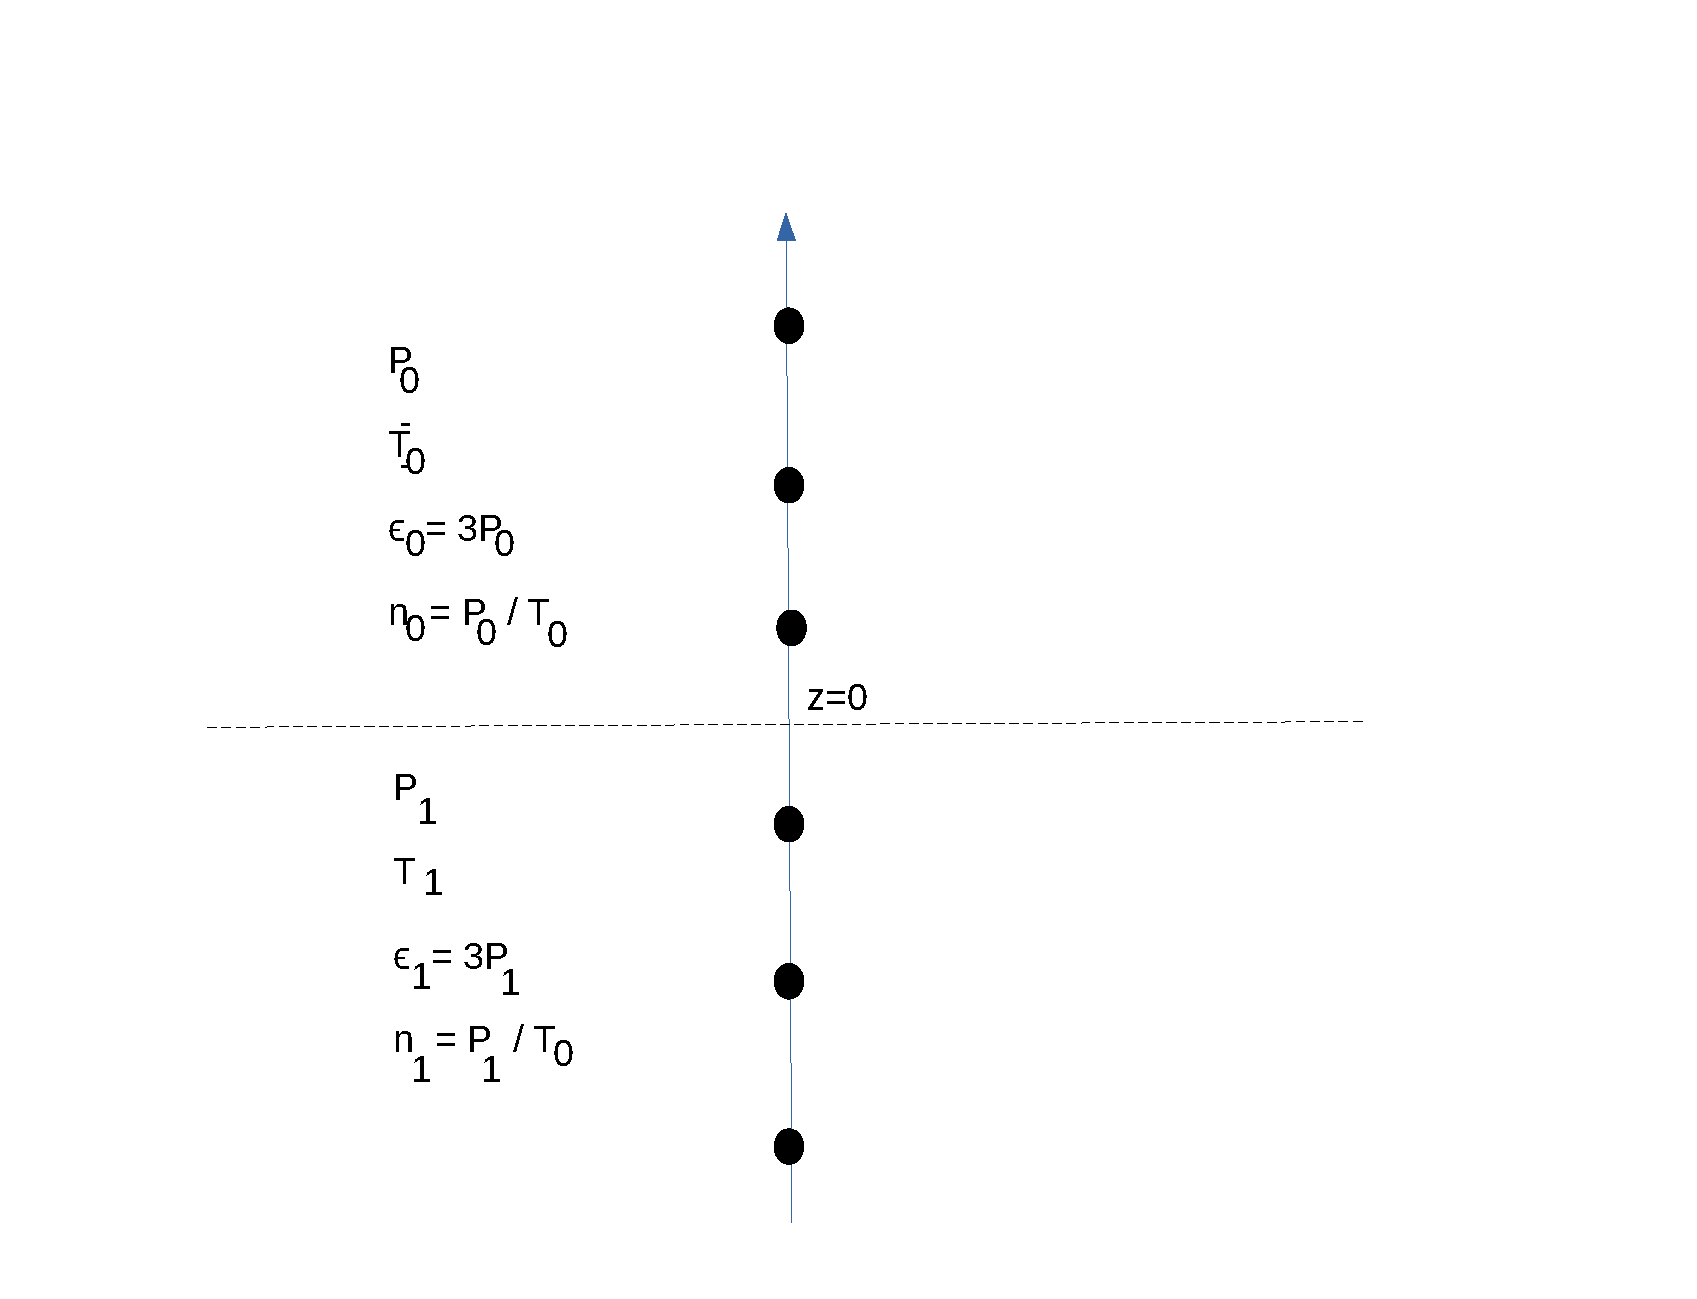
\includegraphics[scale=0.42]{riemann1d.pdf}
\caption{Esquema del problema de riemann en 1-D con valores de P diferentes en cada semisegmento.}
\end{figure}
 
 Se implementa una simulación uno-dimensional\footnote{riemann1D.cpp} con un arreglo de tamaño $1\times1\times800$. Para ello se utiliza el set de velocidades $D1Q3$, con las velocidades $\vec{c}_0=0$, $\vec{c}_1=+1$, $\vec{c}_2=-1$, y cuyos pesos están dados por $w_0=2/3$, $w_1= w_2= 1/6$, respectivamente. Se inicializan los valores de las funciones de distribución, densidades de energía y de número de partículas, y velocidades en $z$ como
  \begin{subequations}
\begin{equation}
   v_z=0,\ \ \longrightarrow \gamma =1,
\end{equation}
\begin{equation}
    \epsilon = 3P,
\end{equation}
\begin{equation}
    n = \frac{P}{T_0},
\end{equation}
con $P$ diferente dependiendo de cada región y $T=T_0$ la misma en todo el dominio.
\end{subequations}
Con esta inicialización se cumplen las constricciones macroscópicas de la Ec. (6).\\

En este caso 1-D, la 4-velocidad está dada por $u^{\mu}= (\gamma, 0, 0, \gamma \beta)^{\mu}$, con $\beta = |\vec{u}|/c$. Además, se utiliza la velocidad de red dada por $c_l=1.0$. Los valores de la presión fueron elegidos como $P_0= 7.9433\times 10^{-6}$ y $P_1= 3.2567\times 10^{-6}$, mientras que la tamperatura inicial es $T_0= 0.0287$, todas ellas en unidades numéricas.\\

 La viscosidad cortante se calcula como 
 \begin{equation}
\eta = \frac{4}{9} \gamma \epsilon (\tau-\delta t /2) c_l^2,
 \end{equation}
 mientras que la entropía se calcula mediante la aproximación 
 \begin{equation}
     s= 4n - n\text{ln} \lambda,
 \end{equation}
 con $\lambda = \frac{n}{n^{eq}}$ la fugacidad del gluón, donde la densidad de partículas en equilibrio está dada por $n^{eq}= \frac{d_G T^3}{\pi^2}$ con $d_G=16$ para gluones. De estas dos cantidades (viscosidad y entropía) se obtiene su radio, $\eta/s$, que será utlilizado como prámetro en la simulación.\\
 
 En los dos bordes de la cadena uno-dimensional se aplican condiciones de frontera abierta. Existen diferentes formas de aproximar dichas condiciones de frontera mediante la extrapolación de poblaciones conocidas, algunas de ellas son\footnote{mohammad}:
 
\begin{itemize}
    \item \textbf{Extrapolación a primer orden}\\
    Borde superior: 
    \begin{equation}
        f_{2, N_z-1} = f_{2, Nz-2}.
    \end{equation}
    Borde inferior:
    \begin{equation}
        f_{1, 0} = f_{1, 1}.
    \end{equation} 
    
    \item \textbf{Extrapolación a segundo orden}\\
    Borde superior: 
    \begin{equation}
        f_{2, N_z-1} = 2f_{2, Nz-2}- f_{2, Nz-3}.
    \end{equation}
    Borde inferior:
    \begin{equation}
        f_{1, 0} = 2f_{1, 1}-f_{1, 2}.
    \end{equation} 
\end{itemize}
Otra alternativa es asumir que la presión es conocida en la frontera, y por lo tanto $\epsilon$ y $n$. Se fijan los valores de las densidades a algún valor, por ejemplo a $1.0$. Si por ejemplo, se conoce la presión a la salida, se obtienen las ecuaciones para el borde superior
\begin{subequations}
\begin{equation}
    u_z = 1 - \frac{2f_{1, Nz-1} + f_{0, Nz-1}}{n_{outlet}},
\end{equation}
\begin{equation}
    f_{2,Nz-1} = f_{1, Nz-1} - \frac{2}{3} n_{outlet}u_z.
\end{equation}
\end{subequations}
Para el borde inferior
\begin{subequations}
\begin{equation}
    u_z = -1 + \frac{2f_{2,0} + f_{0,0}}{n_{outlet}},
\end{equation}
\begin{equation}
    f_{1,0} = f_{2,0} - \frac{2}{3} n_{outlet}u_z.
\end{equation}
\end{subequations}

\end{document}